\begin{circuitikz}[background rectangle/.style={fill=white}, show background rectangle]
        \node(0,0) {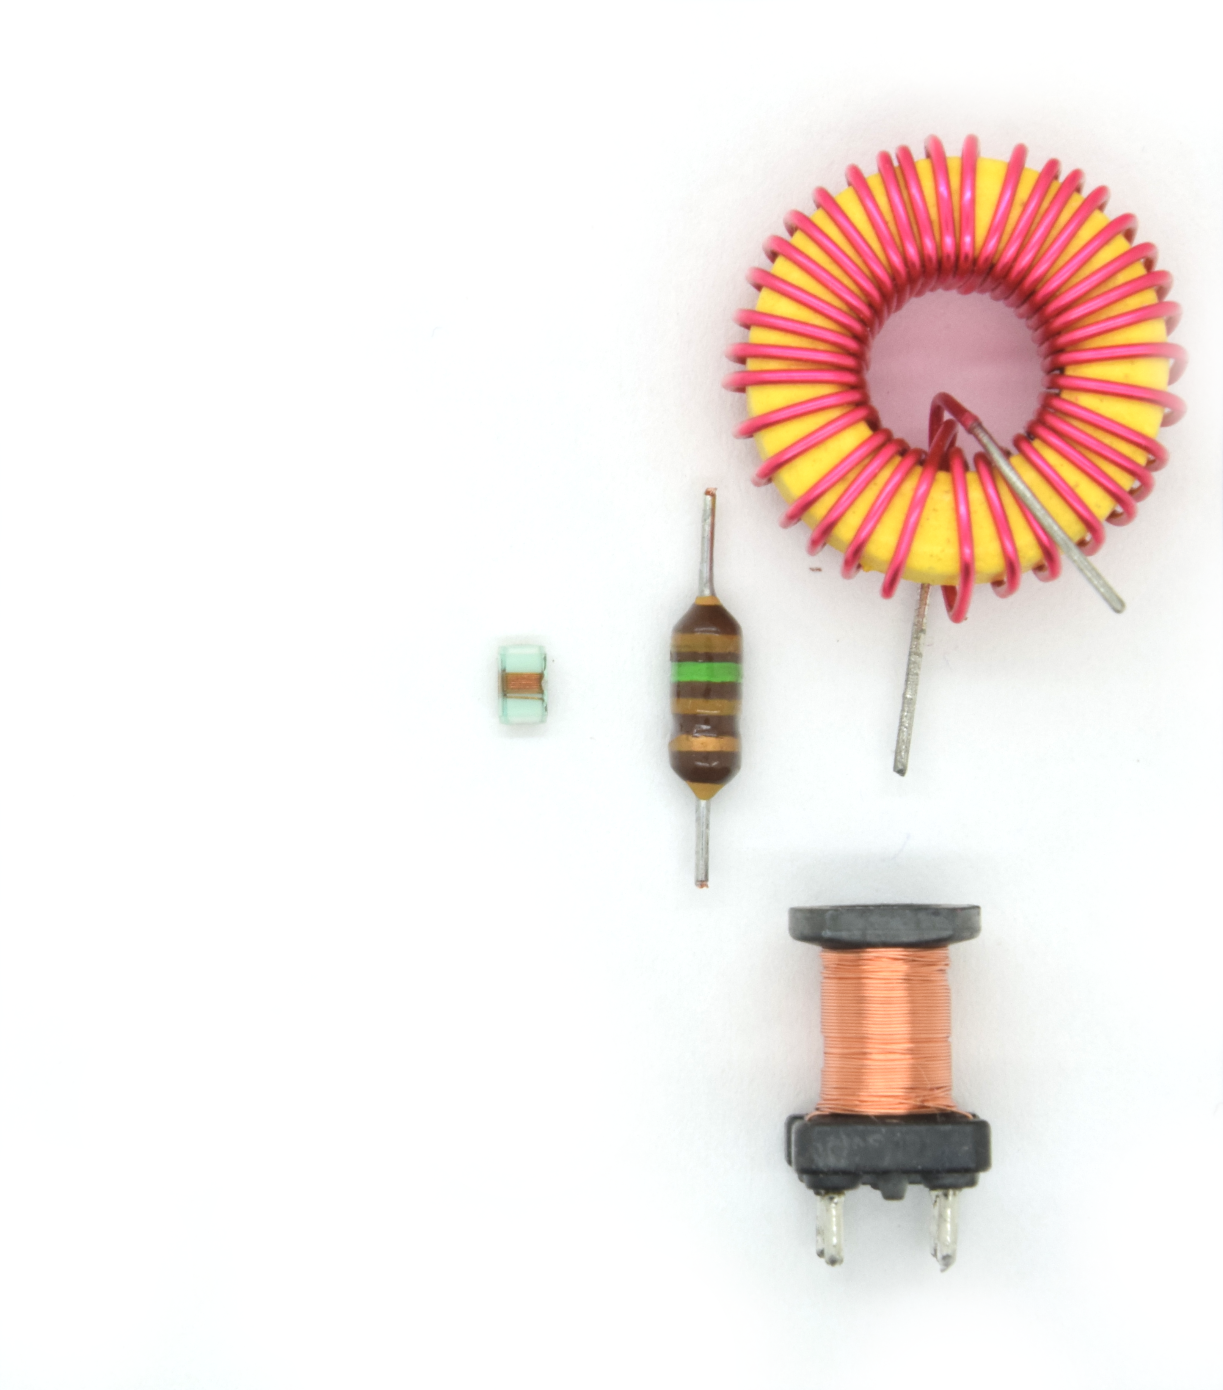
\includegraphics[width=200pt]{foto/9}};
        
        \draw(-3.0,1) to [L, american,l={$L$}] ++(0,-2);
    
        % Beschriftung:
        \draw( 2.15,  3.50) node {\small \qty{47}{\micro\henry}};
        \draw( 2.35,  0.25) node {\small \qty{3}{\ampere}};
        \draw( 0.55, -1.85) node[rotate=90] {\small \qty{150}{\micro\henry}};
        \draw( 1.55, -3.75) node {\small \qty{5}{\milli\henry}};
        \draw(-0.50,  0.45) node[right, rotate=90] {\small PLCC2 \qty{100}{\nano\farad}};
    
        % Pfeile:
        \draw[>=triangle 60, <->] (-1.6,0.675) coordinate(c1) -- ++(0,-1.35) coordinate(c2);
        \draw(c1) -- ++( 0.25,0);
        \draw(c1) -- ++(-0.25,0);
        \draw(c2) -- ++( 0.25,0);
        \draw(c2) -- ++(-0.25,0);
    
        % Text:
        \draw (c1) ++ (0,0.25) node {\qty{1}{\centi\meter}};
    
\end{circuitikz}